\section{Related Work}
\label{sec:related}

\begin{figure}[t!]
\begin{minipage}{\textwidth}
  \centering
  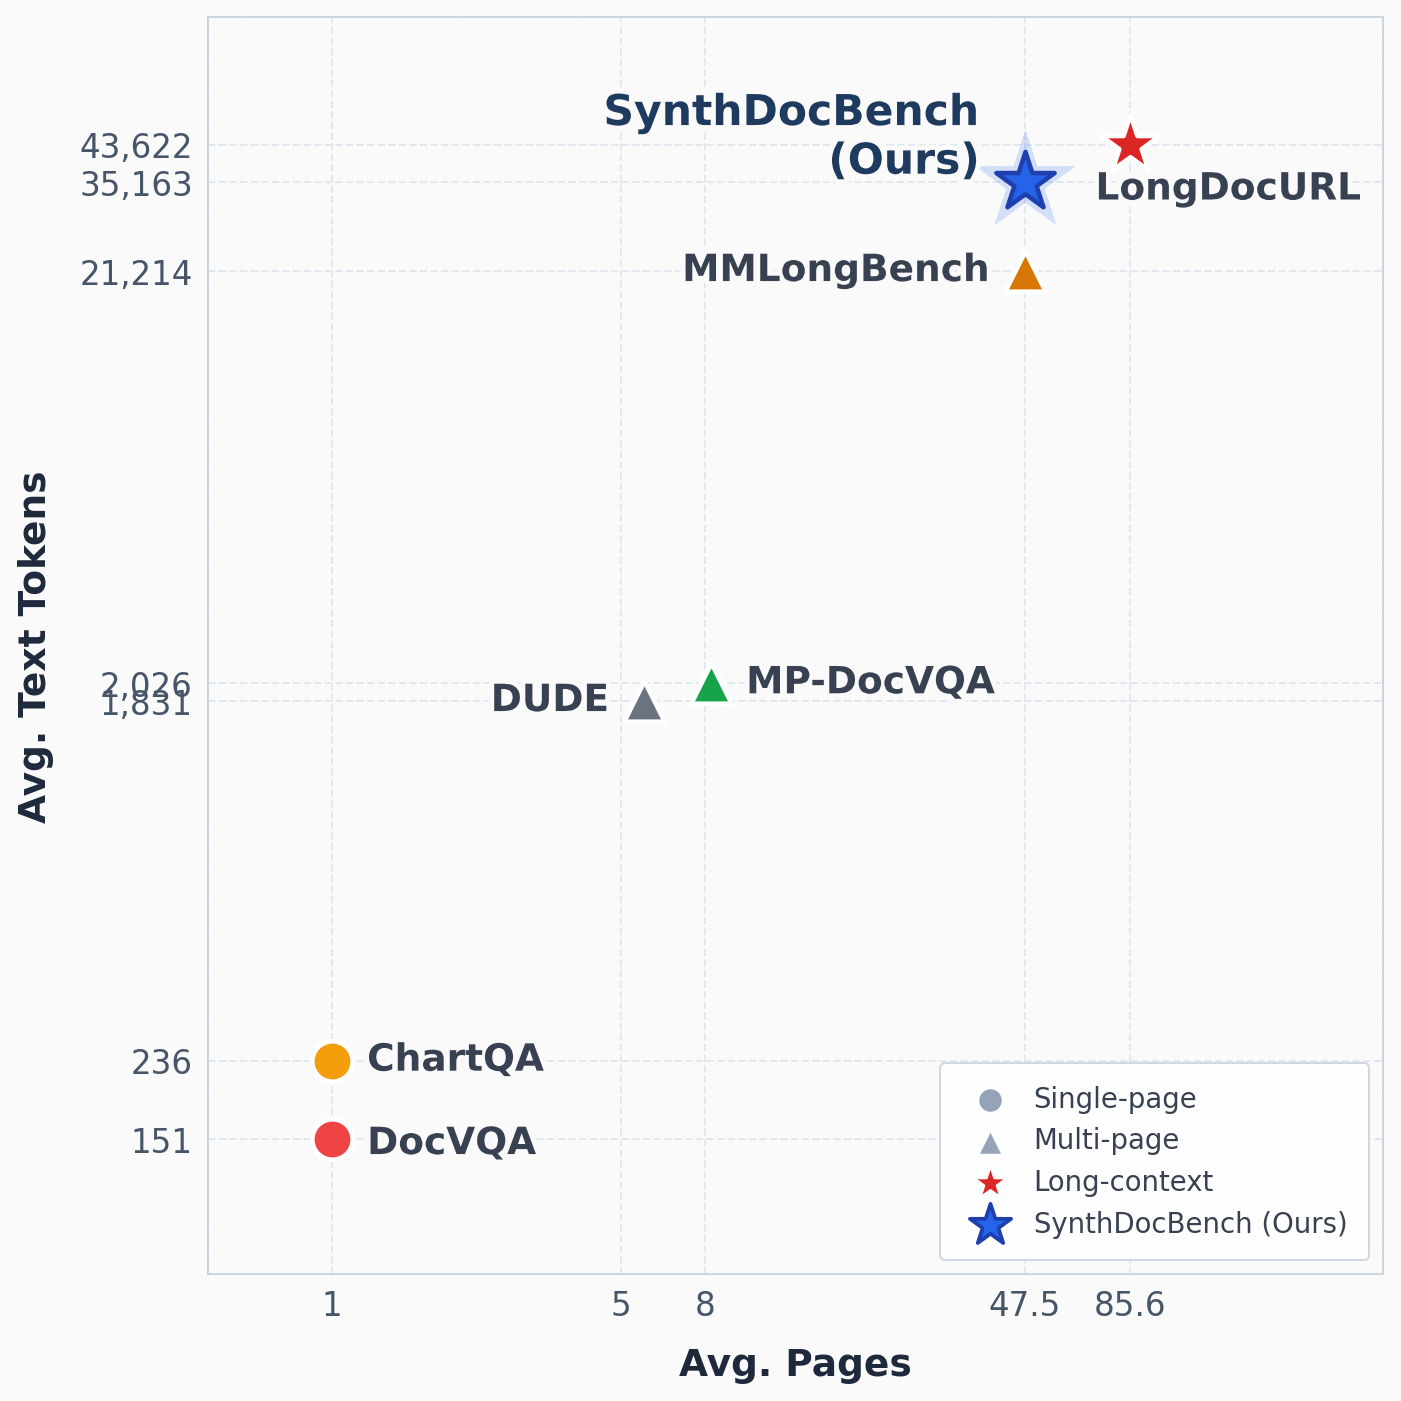
\includegraphics[width=0.55\textwidth]{images/benchmark_plot.png}
\end{minipage}

\vspace{14pt}

\begin{minipage}{\textwidth}
  \centering
  \footnotesize
  \resizebox{\textwidth}{!}{%
  \begin{tabular}{@{}lcccc@{}}
  \toprule
  \textbf{Benchmark} & \textbf{Scope} & \textbf{Avg.\ Context} & \textbf{\#Docs/Charts} & \textbf{\#Questions} \\
  \midrule
  \rowcolor{gray!15} \multicolumn{5}{c}{{Chart Benchmarks}} \\
  \midrule
  ChartQA \citep{masry2022chartqa}               & Isolated charts   & 1 chart       & 21,953    & 32,701 \\
  ChartQAPro \citep{masry2025chartqapro}         & Isolated charts   & 1 chart       & 1,341     & 1,948  \\
  ChartGalaxy \citep{li2025chartgalaxy}          & Isolated charts   & 1 chart       & 1,763,189 & ---    \\
  VisuLogic \citep{zhang2025visulogic}           & Isolated images   & 1 image       & 1,000     & 1,000  \\
  ChartMuseum \citep{xu2025chartmuseum}          & Isolated charts   & 1 chart       & 928       & 1,162  \\
  MultiChartQA \citep{zhu2025multichartqa}       & Multi-chart       & 2--3 charts   & 655       & 944    \\
  \midrule
  \rowcolor{gray!15} \multicolumn{5}{c}{{Document VQA Benchmarks}} \\
  \midrule
  DocVQA \citep{mathew2021docvqa}                & Single-page docs  & 1 page        & 12,767    & 50,000 \\
  MP-DocVQA \citep{tito2023hierarchical}         & Multi-page docs   & $\leq$20 pages & ---      & 46,000 \\
  SlideVQA \citep{tanaka2023slidevqa}            & Multi-page docs   & $\sim$20 pages & 2,619    & 14,500 \\
  MMLongBench-Doc \citep{ma2024mmlongbenchdoc}   & Multi-page docs   & 47.5 pages    & 135       & 1,082  \\
  LongDocURL \citep{deng2025longdocurl}          & Multi-page docs   & $\sim$83 pages & 396      & 2,325  \\
  M-LongDoc \citep{chia2024mlongdoc}             & Multi-page docs   & $>$200 pages  & ---       & 851    \\
  MMLongBench \citep{wang2025mmlongbench}        & Multi-page docs   & 8K--128K tokens & 13,331  & ---    \\
  \midrule
  
\includegraphics[width=0.8em]{images/icon2.png} \textbf{\textsc{SynthDocBench}} & \textbf{Multi-page docs} & \textbf{Avg.\ 51.1 pages} & \textbf{200 / 3,340} & \textbf{1,788} \\
  \bottomrule
  \end{tabular}
  }
  % \captionof{table}{Benchmarks in chart reasoning and long-context document understanding. ChartGalaxy and MMLongBench do not report \#Questions; MP-DocVQA and M-LongDoc do not report doc counts.}
\end{minipage}
\vspace{-6pt}
\caption{\textbf{Landscape of benchmarks} 
Top: benchmark comparison by average document length (pages) and average textual context (tokens). SynthDocBench occupies a unique region with both long multi-page context and high textual density.
Bottom: comparison with existing chart and document VQA benchmarks. 
Prior benchmarks typically isolate either charts or long documents, whereas \textbf{\textsc{SynthDocBench}} is designed to study their intersection under long contexts.}
\label{fig:related_benchmarks}
\end{figure}

\subsection{Charts and Visual Reasoning}

% Charts and tables constitute among the most inferentially demanding element types encountered in professional documents, yet their evaluation has proceeded largely in isolation from the long-context document setting in which they most commonly appear. ChartQA~\citep{masry2022chartqa} established the methodological foundation for chart-oriented visual question answering, treating charts as standalone images paired with targeted questions. Whilst this paradigm has driven substantial progress, it is now approaching saturation, with frontier models such as Claude Sonnet 4.5~\citep{anthropic2024claude35sonnet} attaining 89.0\% accuracy and open source models like Qwen3-VL 235B~\citep{bai2025qwen3} attaining 91.2\%. Furthermore, it abstracts away the document context in which charts are encountered in practice. ChartQAPro~\citep{masry2025chartqapro} addresses the saturation problem through harder and more diverse real-world charts, with models that saturate ChartQA exhibiting performance degradation in excess of 30 percentage points. However, it retains the isolated-image paradigm. ChartGalaxy~\citep{li2025chartgalaxy} demonstrates that programmatic generation can yield million-scale synthetic diversity spanning 75 chart types and 330 stylistic variations, providing a methodological precedent for the synthetic approach adopted in \textsc{SynthDocBench}, though again without embedding charts within multi-page document contexts. VisuLogic~\citep{zhang2025visulogic} and ChartMuseum~\citep{xu2025chartmuseum} probe fine-grained logical and perceptual reasoning over isolated charts, exposing failure modes that aggregate accuracy on ChartQA does not surface; and MultiChartQA~\citep{zhu2025multichartqa} extends the paradigm to reasoning across several charts presented simultaneously. Taken together, these benchmarks establish that chart understanding is far from solved, yet none model the setting in which a chart must be interpreted in conjunction with the surrounding prose, tables, and figures of a multi-page document. \textsc{SynthDocBench} is designed to evaluate precisely the capability of VLMs to reason over relevant context which can be spatially distant from the chart itself and needs retrieval and understanding spanning multiple pages.

\subsection{Long-Context Multimodal Benchmarks}


% Evaluation of long-context understanding of Vision Language Models (VLMs) has progressed from shallow retrieval paradigms toward tasks demanding multi-step reasoning and cross-modal synthesis. Early evaluation focused on needle-in-a-haystack (NIAH) settings~\citep{wang2024mmniah}, assessing whether a model can locate a single planted fact within a long context. While operationally straightforward, such probes  the difficulty ceilings in these settings are insufficient to study frontier models, and retrieval accuracy constitutes a poor proxy for downstream reasoning performance~\citep{wang2025mmlongbench}.

% Document-centric benchmarks represent the most directly relevant line of prior work.
% DocVQA~\citep{mathew2021docvqa} established single-page document visual question answering as a standard evaluation task. 
% Its multi page extension MP-DocVQA~\citep{tito2023hierarchical}, and the presentation-oriented 
% SlideVQA~\citep{tanaka2023slidevqa} broadened scope to multi-image documents. However, both benchmarks are nonetheless constrained to documents averaging fewer than approximately twenty pages and principally assess span extraction rather than inferential reasoning, with charts and figures playing a limited evidential role in the required reasoning chain. 

% MMLongBench-Doc~\citep{ma2024mmlongbenchdoc} constituted the first benchmark to target long PDF comprehension ($>$47 average pages per document) with rich visual content including charts, tables, and figures interleaved with text, requiring models to synthesize evidence distributed across multiple pages.
% MMLongBench~\citep{wang2025mmlongbench} extended this framework to five task categories spanning 8K to 128K token contexts, demonstrating that long-document VQA yields the most stable and discriminative signal among the task categories examined, and that performance on retrieval-oriented sub-tasks correlates poorly with that on reasoning sub-tasks. This finding indicates that aggregate scores overshadow qualitatively distinct failure modes.
% LongDocURL~\citep{deng2025longdocurl} and M-LongDoc~\citep{chia2024mlongdoc} represent the most closely related prior work, advancing the state of the art through cross-element localisation tasks and open-ended explanatory responses over documents spanning several hundred pages. 

% Nonetheless, both benchmarks are primarily oriented toward breadth of coverage, maximizing the range of document types, task categories, and page counts rather than toward diagnostic decomposition of model failure modes. While LongDocURL categorizes chart and figure content as one of four evidence types, the majority of questions require a single point of extraction from a localized document region.  M-LongDoc similarly emphasizes retrieval over long documents as its primary evaluative challenge, with its principal contribution being a tuning framework rather than a controlled diagnostic instrument. Neither benchmark constructs questions that specifically require reasoning over multiple charts in conjunction with contextually related evidence distributed across distant pages. \textsc{SynthDocBench} is distinguished from both by its explicitly diagnostic intent, it varies document length, page depth, modality composition, and question type as independent axes, and specifically foregrounds charts and figures as primary reasoning targets, with questions constructed to require their interpretation alongside prose and tabular evidence that may be arbitrarily distant within the document.

\subsection{Vision-Language Models for Document Understanding}

% The rapid capability growth of vision-language models (VLMs) across document understanding tasks is itself a primary motivation for the present work. On single-page benchmarks such as DocVQA, frontier open source models including Qwen3-VL~\citep{bai2025qwen3} and InternVL3.5~\citep{wang2025internvl3} now approach or exceed 95\%, rendering these evaluations largely uninformative for discriminating among leading systems. Performance on the more demanding ChartQA similarly approaches saturation. However, progress on long-context benchmarks is considerably more constrained: on MMLongBench-Doc, the best-performing model currently (Qwen3-VL) achieves accuracy 57\%\footnote{\url{https://huggingface.co/spaces/OpenIXCLab/mmlongbench-doc} bandleader accessed March 2026}.

% Figure~\ref{fig:benchmark_comparison} visualises the landscape of document VQA
% benchmarks along two axes: average document length (pages) and average token
% count per document. Single-page benchmarks (DocVQA, ChartQA) occupy the
% bottom-left, while multi-page benchmarks cluster toward the right.
% \textsc{SynthDocBench} sits at the frontier of both axes among multi-page
% benchmarks---comparable to LongDocURL in page count and substantially richer
% in token density than MMLongBench---while being the only benchmark in this
% space built entirely from controlled synthetic documents.
%%%% , and on MMLongBench even the strongest model (Gemini-2.5-Pro, leading open-source counterparts by approximately 20 points \footnote{As presented in \cite{wang2025mmlongbench} - leaderboard unavailable as of March 2026}) achieves an average of 77.2 at the 128K token context length across 5 tasks. \textcolor{red}{average is taken over some tasks not relevant for us, so this number is misleading}
% This performance gap between single-page and long-context settings indicates that long-context visual document reasoning constitutes a substantively unsolved problem for current VLMs, and that the diagnostic signal available from existing benchmarks remains insufficient to identify the specific document properties and reasoning demands responsible for observed failures - a gap which \textsc{SynthDocBench} is designed to address.


% _____________
% \subsection{Synthetic Benchmarks and Controlled Evaluation}

% The use of synthetic data for controlled evaluation is well established in
% NLP\cite{weston2015babi, lake2018scan} but remains rare in multimodal document
% understanding. \textbf{MMLongBench-Doc} employs semi-synthetic PDFs but does not
% systematically vary document properties. \textbf{ChartGalaxy}\cite{li2025chartgalaxy}
% generates charts programmatically to achieve scale and diversity, yet restricts
% attention to isolated chart images rather than full document contexts.

% \textsc{SynthDocBench} is the first benchmark to apply fully factorial synthetic
% generation to long-context visual document understanding. Four axes---document
% length, page depth, modality composition, and question type---are varied
% independently across documents generated by an end-to-end LLM pipeline, enabling
% the first clean decomposition of MLLM failure modes. This design eliminates the
% confounds inherent in real-document benchmarks and yields interpretable signal about
% precisely \textit{what} models are failing at and \textit{why}.

